\documentclass[11pt]{article}
\usepackage[utf8]{inputenc}
\usepackage{graphicx}
\usepackage{verbatim}
\usepackage{listings}
\lstset{language=C, frame=single}

\topmargin=-15mm
\oddsidemargin=0mm
\textwidth=159.2mm
\textheight=220mm

\title{Motion JPEG Encoding on Intel x86 using Streaming SIMD Extensions (SSE)}
\author{Paweł Kozłowski \and Łukasz Mazurek}


\begin{document}
\maketitle

\section{Introduction}
TODO

\section{Optimalizations}

\begin{figure}[h]
	\centering
	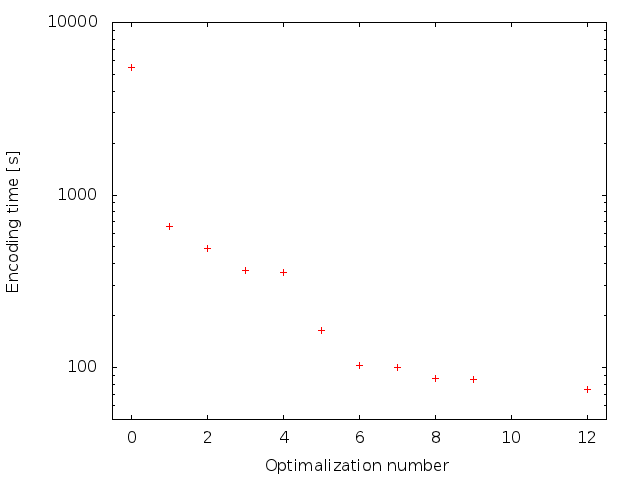
\includegraphics[width=0.7\textwidth]{img/times.png}
	\caption{Time of encoding \texttt{tractor.yuv} movie. After 12 optimalizations this time was reduced from 5475s to 74.6s}
	\label{times_plot}
\end{figure}

We have implemented 12 optimalizations of \texttt{mjpeg\_encoder} program.
In the fig. \ref{times_plot} we can see time of encoding the movie\footnote{All times used in this report are times of encoding \texttt{tractor.yuv} on \emph{Clinton} machine.} after each optimalization.
All optimalizations together have reduced this time by factor 73.4, from 5475s to 74.6s. 

\subsection{Opt 1: Cosine array}
We recognized that first bottleneck (83.7\% of samples) is this line:

\begin{lstlisting}
dct += coeff * (float) (cos((2*i+1)*u*PI/16.0f) 
     * cos((2*j+1)*v*PI/16.0f));
\end{lstlisting}
It contains slow computing of \emph{cos} function.
Since \texttt{i}, \texttt{u}, \texttt{j} and \texttt{v} are integers between 0 and 7, there are only 64 possible arguments of this \emph{cos}.
Therefore we can calculate the values of 
$$\cos \frac{(2a + 1) b \pi}{16}$$
once, for all $a, b \in \{0, \ldots, 7 \}$ and store them in array \texttt{cos\_table[8][8]}.
After that we can get the value of \emph{cos} function from the array instead of computing it every time.
Thus, considered line changed to:
\begin{lstlisting}
dct += coeff * cos_table[i][u] * cos_table[j][v];
\end{lstlisting}

Optimalization described above improved \texttt{mjpeg\_encoder} by factor 8.3, from 5475s to 657.8s.

\subsection{Opt 2: Products of cosines array}
Next observation: since there is only 64 possible values of $\cos$ function,
there is only $64 \cdot 64 = 4096$ possible values of product of two cosines.
Therefore we can store in array values of products
$$\cos \frac{(2a + 1) b \pi}{16}
\cos \frac{(2c + 1) d \pi}{16}$$
for all $a, b, c, d \in \{0, \ldots, 7 \}$.
Now considered line changed to:
\begin{lstlisting}
dct += coeff * cos_table[i][u][j][v];
\end{lstlisting}
This optimalization improved program speed by factor 1.34, from 657.8s to 490.1s.

\subsection{Opt 5: SSE multiplying}
After first two optimalizations the bottleneck was the floating-point addition and multiplication in following lines:
\begin{lstlisting}
float coeff = in_data[(y+j)*width+(x+i)] - 128.0f;
dct += coeff * cos_table[i][u][j][v];
\end{lstlisting}
Firstly, we changed these arithmetic operations from \texttt{float} to \texttt{int} operations, what improved program by factor 1.34, 
but finally we decided to come back to \texttt{float} numbers and change operations to \emph{SSE} addition and multiplication:
\begin{lstlisting}
__m128 coeff = _mm_load_ps(in_ptr);
__m128 cos_4float = _mm_load_ps(cos_ptr);

coeff = _mm_sub_ps(coeff, M128);
coeff = _mm_mul_ps(coeff, cos_4float);
_mm_store_ps(table, coeff);
dct += table[0] + table[1] + table[2] + table[3];

cos_ptr += 4;
in_ptr += 4;
\end{lstlisting}
Therefore we were doing 4 substractions at once and 4 multipications at once.
This change improved the code 3 times, from 490s to 164s.

The problem was that \texttt{in\_data} was the type of \texttt{uint8\_t}
and was multiplied by \texttt{float} cosine.
At first we implemented a trick with casting \texttt{uint8\_t} to (m64) TODO:

TODO

Unfortunately, this trick didn't work on \emph{Clinton} machine, 
so we decided to change the type of \texttt{in\_data} to \texttt{float}.

\section{Opt 6: Multiplication and addition -> dot product}
The next bottleneck was an addition of 4 \texttt{float}s.
This \texttt{float}s were results of multiplication 4 consecutive elements
of \texttt{in\_data} array and cosine array.
\begin{lstlisting}
coeff = _mm_mul_ps(coeff, cos_4float);
_mm_store_ps(table, coeff);
dct += table[0] + table[1] + table[2] + table[3];
\end{lstlisting}
We can do multiplication of four pairs of floats and sum up the results
in one \emph{SSE} operation: \textbf{dot product}:
\begin{lstlisting}
coeff = _mm_dp_ps(coeff, cos_4float, 0xf1);
_mm_store_ss(table, coeff);
dct += table[0];
\end{lstlisting}
This optimalization improved code by factor 1.6 to 103s total time.

\section{Opt 7: Load operation moved out from a loop}
We recognized that \texttt{\_mm\_load\_ps} operation of input data 
is performed $64 \cdot 16$ times for each block.
\begin{lstlisting}
__m128 coeff = _mm_load_ps(in_ptr);
\end{lstlisting}
Since there are only 16 different values of possible input data to load
in a certain block, we can load it once and store in 16 registers:
\begin{lstlisting}
__m128 c[16];
for (i = 0; i < 16; i += 2) {
    c[i] = _mm_load_ps(in_ptr);
    c[1+1] = _mm_load_ps(in_ptr + 4);
    in_ptr += width;
}
\end{lstlisting}
This optimalization improved program only by factor 1.03.

\section{Opt 8 and 9: \texttt{float()} function removed and \texttt{uint8\_t quantization} -> \texttt{float quantization}}
The next bottleneck was in the following line:
\begin{lstlisting}
out_data[(y+v)*width+(x+u)] = 
  (int16_t)(floor(0.5f + dct / (float)(quantization[v*8+u])));
\end{lstlisting}
Of course \texttt{floor} operation before casting to \texttt{int16\_t}
is unnecessary here, so we can just remove it.
Other slow operation in this line is casting \texttt{uint8\_t quantization} array to \texttt{float}.
Since \texttt{quantization} is a constant array $8 \times 8$ we can store it
in memory as a \texttt{float} array and avoid this casting each time.
These two changes improved our encoder by factor 1.18.

\section{Opt 13: Cos + malloc}
This time profiling showed that line:
\begin{lstlisting}
*out_ptr = (int16_t)(0.5f + tmp[v * 8 + u] / (quantization[v*8+u]));
\end{lstlisting}
It turned out that this division can be done once in the beginning
with each computated $\cos$ value.

Next thing was change in frequency of using \texttt{malloc()} function,
we can of course call it once per program run, not once per frame.

This optimizations improved our code by factor 1.10, from 83.6s to 76.0s.


\section{Opt 12: Zmiana koncepcji?}
Until now we were using more than 16 variables of \_\_m12 type8,
so there probably were problems with switching data in registers.
We changed completely order of computations. From now on we compute
firstly all things related to first row of input data and then go
to next row of input data. It forces us to keep out data in local
variable and sum up data from each input row. It allows us to use
about 5 variables of \_\_m128 type, so there is no problem with
switching data in XMM registers any more. This optimalization
improved our code by factor 1.02, from 76.0s to 74.5s. This shows
that compiler makes really good optimizations.

\end{document}
